\section{Experiment 3 : The errors-in-variables method}
For the first experiment, we use the following parameter settings : 

\begin{table}[h]
\centering
\begin{tabular}{ll}
    $ R_0 = 1000, $  &  $ sigma_{n_i} = 0.001, $   \\
    $ \sigma_{i_0} = 0.01, $  &  $ \sigma_{n_u} = 1, $   \\
\end{tabular}
\end{table}
The result of the first experiment are displayed on the figure~\ref{Sess1_part1_exp1}.

\paragraph{LS estimator} As can be seen on the top picture of fig.~\ref{Sess1_part1_exp1}, the LS estimate is biased. This bias is due to the fact that, with the LS estimate, we assume that the measured input is exact, which is not the case here because of the noise $n_i$. The relative bias is 1\% which is not large but still a bias.

TODO: try to express this as a function of the given parameter settings

\paragraph{EIV estimator} The EIV estimator has a mean of about 1000.1. Which means it has a bias of about 0.1\%. This bias will vanish if we increase the amount of experiments.

TODO: would the IV estimator work here?

\begin{figure}[H]
    \centering
    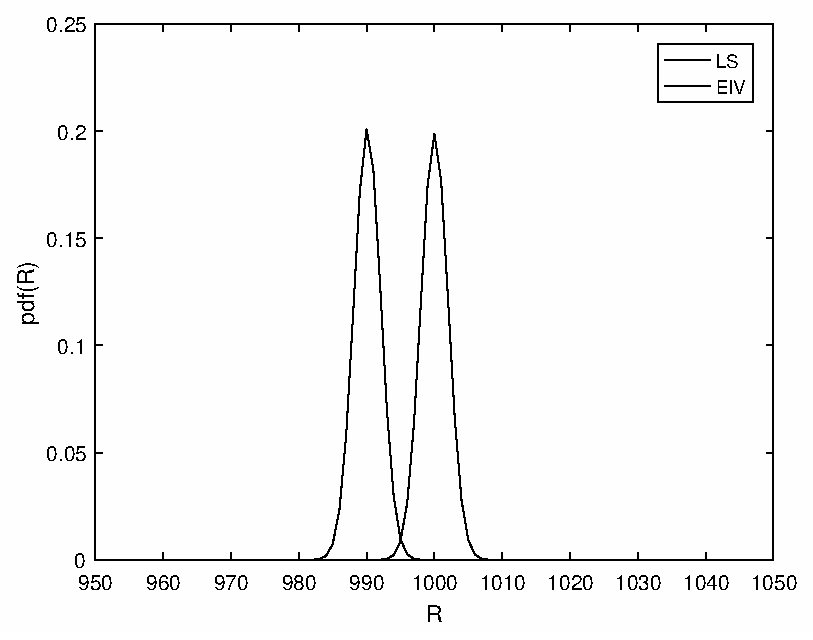
\includegraphics[width=1\textwidth]{Figures/Sess1_part2.eps}
    \caption{Comparison of the PDF of the LS and EIV estimate, calculated with prior known variables}
    \label{Sess1_part1_exp1}
\end{figure}

